\chapter{Strumenti Utilizzati}

\section{Introduzione}
    In questo capitolo verranno introdotti gli strumenti utilizzati per affrontare la tesi, in particolare ci si concentrerà su: \texttt{MNIST}, \texttt{PyTorch} e \texttt{DEAP}.


\section{MNIST}
Il dataset MNIST (Modified National Institute of Standards and Technology) è uno dei dataset più noti e utilizzati nel campo del machine learning e del riconoscimento di immagini scritte a mano. Esso contiene immagini in scala di grigi di dimensione $28 \times 28$ pixel rappresentanti cifre da 0 a 9, quindi ogni immagine ha una singola componente di colore e può essere rappresentata come un tensore con shape $(1,28, 28)$.  
\\MNIST è composto da 60.000 immagini per il training e 10.000 immagini per il testing, ed è particolarmente utile per sperimentare algoritmi di classificazione perché le immagini sono già normalizzate e centrate. Ogni immagine è accompagnata da un’etichetta che indica quale cifra rappresenta (da 0 a 9), rendendo il dataset un tipico problema di classificazione supervisionata a 10 classi.  
\\Il dataset è stato originariamente derivato dal NIST, ma successivamente è stato preprocessato e ridimensionato da LeCun et al. per rendere le immagini più uniformi e facilmente utilizzabili dagli algoritmi di machine learning. La semplicità e la standardizzazione di MNIST lo rendono ideale per testare nuovi modelli, confrontare algoritmi di ottimizzazione e valutare rapidamente la capacità di una rete neurale di apprendere rappresentazioni visive.  
\begin{figure}[h!]
    \centering
    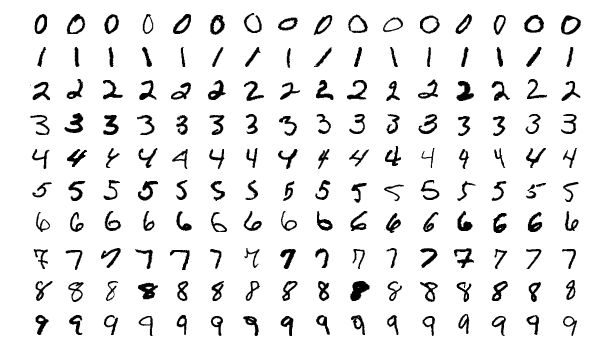
\includegraphics[width=0.5\textwidth]{img/MnistExamples.png}
    \caption{Dataset MNIST. Immagine tratta da \cite{MNIST_Examples_Image}}
    \label{fig:Dataset_MNIST}
\end{figure}

\section{PyTorch}

PyTorch è un framework open-source per il deep learning sviluppato dal laboratorio \textit{Facebook AI Research} (FAIR) e rilasciato per la prima volta nel 2016. Negli anni è diventato uno degli strumenti più diffusi sia in ambito accademico che industriale, grazie alla sua semplicità, alla grande flessibilità e all'approccio dinamico alla costruzione dei modelli. A differenza di altri framework che utilizzano un grafo statico, PyTorch si basa su un \textit{dynamic computation graph}, che permette di modificare la struttura della rete durante l'esecuzione, risultando molto utile nella fase di prototipazione e ricerca.

\subsection{Concetti Fondamentali}
Gli elementi principali su cui si fonda PyTorch sono:
\begin{compactitemize}
    \item \textbf{Tensori}: strutture dati multidimensionali, simili agli array NumPy, ma ottimizzate per il calcolo parallelo e in grado di sfruttare GPU e CPU in modo trasparente.
    \item \textbf{Autograd}: un sistema di differenziazione automatica che registra tutte le operazioni eseguite sui tensori e consente di calcolare i gradienti necessari per l'ottimizzazione dei parametri.
    \item \textbf{torch.nn}: una libreria che fornisce classi modulari per definire reti neurali, come layer densi (\texttt{nn.Linear}), convoluzionali (\texttt{nn.Conv2d}) o di normalizzazione.
    \item \textbf{torch.optim}: una collezione di algoritmi di ottimizzazione (SGD, Adam, RMSProp) che aggiornano i parametri della rete durante il training.
    \item \textbf{torch.utils.data}: strumenti per gestire dataset e dataloader, che consentono di caricare i dati in batch, applicare trasformazioni e sfruttare il parallelismo.
\end{compactitemize}

\subsection{Definizione delle Reti Neurali}
La costruzione dei modelli in PyTorch si basa sulla classe base \texttt{nn.Module}. Ogni rete neurale viene definita come una sottoclasse di \texttt{nn.Module}, all'interno della quale vengono dichiarati i layer e implementato il metodo \texttt{forward()}, che descrive il passaggio dei dati attraverso la rete.

Ad esempio, un layer completamente connesso (o \textit{fully connected}) viene definito come:
\begin{verbatim}
self.hidden = nn.Linear(512, 256)
\end{verbatim}
dove 512 rappresenta il numero di unità in input e 256 il numero di unità in output.

\subsection{Gestione dei Dati}
PyTorch fornisce strumenti dedicati al caricamento dei dati attraverso le classi \texttt{Dataset} e \texttt{DataLoader}. Queste permettono di:
\begin{compactitemize}
    \item caricare i dati da disco in modo efficiente;
    \item suddividere il dataset in batch;
    \item applicare trasformazioni in tempo reale (ad esempio normalizzazione e data augmentation);
    \item gestire lo shuffling dei dati per migliorare la generalizzazione.
\end{compactitemize}
Grazie al supporto del parallelismo interno, il \texttt{DataLoader} può utilizzare più processi (\texttt{num\_workers}) per caricare i dati in parallelo, riducendo i colli di bottiglia durante l'addestramento.

\subsection{Training e Ottimizzazione}
Il processo di addestramento in PyTorch segue lo schema classico:
\begin{enumerate}
    \item calcolo della \textbf{forward pass} per ottenere l'output della rete;
    \item calcolo della funzione di perdita (es. \texttt{CrossEntropyLoss});
    \item calcolo dei gradienti tramite \textbf{backward pass} (\texttt{loss.backward()});
    \item aggiornamento dei parametri con l'ottimizzatore scelto (\texttt{optimizer.step()});
    \item azzeramento dei gradienti accumulati (\texttt{optimizer.zero\_grad()}).
\end{enumerate}
Questo flusso si ripete per ogni batch di dati fino al completamento delle epoche di training.

\subsection{Parallelismo e Computazione}
Uno degli aspetti più rilevanti di PyTorch è la gestione del parallelismo, sia su \textbf{CPU} che su \textbf{GPU}.

\subsubsection{Parallelismo su CPU}
Quando non è disponibile una GPU, PyTorch sfrutta in modo ottimale la CPU. Internamente, utilizza librerie come \textbf{OpenMP} e \textbf{Intel MKL} per eseguire molte operazioni matematiche in parallelo su più core. 

Inoltre, PyTorch consente di bilanciare due livelli di parallelismo:
\begin{compactitemize}
    \item \textbf{intra-op}: parallelizzazione delle singole operazioni matematiche (es. moltiplicazioni di matrici);
    \item \textbf{inter-op}: parallelizzazione tra operazioni indipendenti.
\end{compactitemize}
Nel contesto degli algoritmi genetici, la valutazione di intere popolazioni di reti può beneficiare del parallelismo multi-processo, ad esempio sfruttando il modulo \texttt{multiprocessing} di Python, dove ciascun processo valuta un sottoinsieme di individui.

\subsubsection{Parallelismo su GPU}
Quando disponibile, PyTorch permette di eseguire i calcoli direttamente su GPU, che sono particolarmente adatte per il deep learning grazie all'elevato numero di core paralleli. L'uso della GPU è reso estremamente semplice: è sufficiente trasferire tensori e modelli sul dispositivo appropriato con:
\begin{verbatim}
device = torch.device("cuda" if torch.cuda.is_available() else "cpu")
model.to(device)
data = data.to(device)
\end{verbatim}
La parallelizzazione su GPU permette di ridurre drasticamente i tempi di addestramento rispetto all'esecuzione esclusivamente su CPU, specialmente per modelli di grandi dimensioni e dataset voluminosi. Tuttavia, nel lavoro descritto in questa tesi, tutti gli esperimenti sono stati eseguiti su CPU.

\subsection{Considerazioni Finali}
PyTorch combina semplicità di utilizzo e potenza computazionale, rendendo agevole sia la prototipazione rapida di nuove architetture sia la loro esecuzione su larga scala. L'uso dei moduli \texttt{nn.Module} e \texttt{nn.Linear}, insieme al sistema \texttt{autograd}, ha reso possibile la definizione di modelli complessi in modo chiaro ed estendibile. Infine, il supporto al parallelismo, sia su CPU che su GPU, lo rende uno strumento estremamente versatile, adattabile a diversi scenari applicativi.


\section{DEAP}
\textbf{DEAP} (Distributed Evolutionary Algorithms in Python) è una libreria open-source scritta in Python, pensata per la costruzione rapida e flessibile di algoritmi evolutivi. È stata sviluppata inizialmente da un gruppo di ricercatori dell'Université Laval in Canada e si è rapidamente affermata come uno degli strumenti più utilizzati in ambito accademico per la ricerca evolutiva e metaeuristica.  
L'obiettivo di DEAP è fornire un insieme di componenti modulari e altamente estendibili, che permetta all'utente di costruire rapidamente algoritmi genetici, strategie evolutive e altre tecniche ispirate alla biologia, senza dover implementare da zero tutti i meccanismi di selezione, mutazione e crossover.

\subsection{Concetti Fondamentali}
La libreria si fonda su alcuni concetti principali:
\begin{compactitemize}
    \item \textbf{Creator}: un modulo che permette di definire tipi personalizzati, come individui e popolazioni, arricchendo oggetti Python (ad esempio liste) con attributi specifici per il problema considerato.
    \item \textbf{Toolbox}: un contenitore in cui vengono registrate tutte le funzioni necessarie all'algoritmo evolutivo, come la generazione degli individui, la funzione di valutazione, le operazioni di crossover e mutazione, e i metodi di selezione.
    \item \textbf{Fitness}: la misura della qualità di un individuo. In DEAP, la classe \texttt{Fitness} è flessibile e può rappresentare sia problemi di massimizzazione che di minimizzazione.
    \item \textbf{Population}: un insieme di individui che evolvono attraverso le generazioni. Una popolazione può essere inizializzata casualmente o derivare da soluzioni già note.
    \item \textbf{Algorithms}: moduli che forniscono implementazioni standard di cicli evolutivi, come \texttt{eaSimple}, \texttt{eaMuPlusLambda}, o \texttt{eaMuCommaLambda}.
\end{compactitemize}

\subsection{Definizione di un Algoritmo Evolutivo}
In DEAP, la costruzione di un algoritmo evolutivo segue tipicamente questi passi:
\begin{enumerate}
    \item definizione della rappresentazione degli individui con il modulo \texttt{creator};
    \item registrazione nel \texttt{toolbox} delle operazioni principali: generazione, valutazione, crossover, mutazione e selezione;
    \item inizializzazione della popolazione;
    \item ciclo evolutivo: valutazione degli individui, selezione dei migliori, applicazione di crossover e mutazione per generare nuove soluzioni;
    \item iterazione fino al raggiungimento del criterio di arresto.
\end{enumerate}

Ad esempio, la definizione di un individuo basato su una lista di numeri reali può essere implementata con:
\begin{verbatim}
creator.create("FitnessMax", base.Fitness, weights=(1.0,))
creator.create("Individual", list, fitness=creator.FitnessMax)
\end{verbatim}
dove \texttt{FitnessMax} indica un problema di massimizzazione.

\subsection{Parallelismo e Computazione Distribuita}
Un aspetto importante di DEAP è il supporto integrato al calcolo parallelo e distribuito. Poiché la valutazione degli individui è spesso la parte più costosa dal punto di vista computazionale, DEAP permette di parallelizzare questa fase attraverso diverse strategie:
\begin{compactitemize}
    \item \textbf{Multiprocessing}: sfruttando il modulo nativo di Python, è possibile distribuire la valutazione degli individui su più core della CPU, riducendo drasticamente i tempi di esecuzione.
    \item \textbf{Parallelizzazione esplicita}: DEAP consente di sostituire la funzione \texttt{map()} standard con versioni parallele o distribuite, ad esempio utilizzando \texttt{multiprocessing.Pool.map} oppure librerie come \texttt{SCOOP} (Scalable Concurrent Operations in Python), che estende il calcolo a cluster e reti distribuite.
\end{compactitemize}
In un contesto come quello della tesi, dove intere popolazioni di reti neurali vengono valutate tramite PyTorch, questo parallelismo è cruciale per accelerare l'esecuzione. Ogni individuo (cioè ogni rete neurale con un diverso set di pesi) può essere valutato in parallelo, riducendo i tempi richiesti per un ciclo evolutivo.

\subsection{Integrazione con PyTorch}
Un vantaggio significativo di DEAP è la sua estrema flessibilità: la funzione di valutazione può essere arbitrariamente complessa e includere strumenti esterni. Nel caso di questa tesi, la valutazione degli individui corrisponde all'addestramento e alla misurazione delle prestazioni di una rete neurale definita in PyTorch.  
Questo consente di unire i due mondi:
\begin{compactitemize}
    \item \textbf{DEAP} gestisce la generazione delle popolazioni, la selezione, il crossover e la mutazione dei parametri;
    \item \textbf{PyTorch} valuta le reti neurali candidate e restituisce la fitness da utilizzare nell'algoritmo evolutivo.
\end{compactitemize}

\subsection{Considerazioni Finali}
DEAP si configura come uno strumento potente e versatile per la sperimentazione di algoritmi genetici. La sua architettura modulare semplifica la costruzione di esperimenti complessi e la sua compatibilità con il calcolo parallelo la rende particolarmente adatta a problemi ad alta intensità computazionale. In combinazione con PyTorch, rappresenta un ambiente ideale per implementare e testare approcci ibridi di addestramento delle reti neurali tramite algoritmi evolutivi.


